\documentclass[12pt]{amsart}

\usepackage{stmaryrd}
\usepackage{enumerate}
\usepackage{epsfig}
\usepackage{amsfonts,amsmath,amssymb,amsthm}

\begin{document} 

\newtheorem{theorem}{Theorem}
\newtheorem{proposition}{Proposition}
\newtheorem{lemma}{Lemma}
\newtheorem{corollary}{Corollary}
\newtheorem{definition}{Definition}
\newenvironment{remark}{\medskip\noindent{\textbf{Remark.}}}{\medskip}
\newenvironment{example}{\medskip\noindent{\textbf{Example.}}}{\medskip}

\newcommand{\cl}{\ensuremath{\prec}}
\newcommand{\cle}{\ensuremath{\preccurlyeq}}

\makeatletter
\newlength{\earraycolsep}
\setlength{\earraycolsep}{2pt}
\def\eqnarray{\stepcounter{equation}\let\@currentlabel%
\theequation
\global\@eqnswtrue\m@th
\global\@eqcnt\z@\tabskip\@centering\let\\\@eqncr
$$\halign to\displaywidth\bgroup\@eqnsel\hskip\@centering
$\displaystyle\tabskip\z@{##}$&\global\@eqcnt\@ne
\hskip 2\earraycolsep \hfil$\displaystyle{##}$\hfil
&\global\@eqcnt\tw@ \hskip 2\earraycolsep
$\displaystyle\tabskip\z@{##}$\hfil
\tabskip\@centering&\llap{##}\tabskip\z@\cr}
\makeatother

\title{Multi-triangulations as complexes of star polygons}
\maketitle

\begin{center}
\textsc{Draft version} - \today
\end{center}
%\begin{abstract}
%\end{abstract}

\section{Introduction}\label{sectionintroduction}

A \emph{$k$-triangulation of a convex $n$-gon} is a maximal set of edges such that no $k+1$ of them mutually cross. Several properties of triangulations have already been generalized to $k$-triangulations, and particularly: 
\begin{enumerate}[(i)]
\item all $k$-triangulations of a convex $n$-gon have the same number of edges \cite{cp-tttccp-92,n-gdfcp-00,dkm-lahp-02};
\item any $k$-triangulation has at least $kn+2k(p-k)$ edges of length less or equal to $p$, for any $k\le p\le \frac{n-1}{2}$ \cite{n-gdfcp-00};
\item any (sufficiently long) edge can be flipped and the graph of flips is regular and connected \cite{n-gdfcp-00,dkm-lahp-02};
\item any $k+1$ consecutive points of a $k$-triangulation of the $(n+1)$-gon can be merged into $k$ points, the incident edges being moved, to obtain a $k$-triangulation of the $n$-gon \cite{n-gdfcp-00,j-gt-03};
\item the set of $k$-triangulations of the $n$-gon is enumerated by a Catalan determinant \cite{j-gt-03,j-gtdfssp-05}.
\end{enumerate}

Surprisingly, as far as we know, there was no direct proofs of (i), (ii) and (iii). Indeed, (i) was always proved assuming (ii) \cite{n-gdfcp-00,dkm-lahp-02}, (ii) was always proved assuming (i), and (iii) was always proved assuming (iv), that is recursively \cite{n-gdfcp-00,j-gt-03}. Furthermore, there was no basic geometric object in $k$-triangulations that correspond to triangles in triangulations. In this paper, we fill this gap.

If $p$ and $q$ are two coprime integers, a \emph{star polygon} of type $\{p/q\}$ is a polygon formed by connecting a set $V=\{s_j\;|\; j\in\mathbb{Z}_p\}$ of $p$ points of the unit circle with the set $E=\{[s_{jq},s_{(j+1)q}] \;|\; j\in\mathbb{Z}_p\}$ of edges that divide the other points into two part of size $q-1$ and $p-q-1$ (see \cite[ pp. 93-95]{c-rp-73}, \cite[pp. 36-38]{c-ig-73} and fig. \ref{starpolygons}). Since they correspond to polygons when we allow crossings, it is natural to think that some star polygons may appear in $k$-triangulations. In fact, the natural generalization of the triangle is the following object:

\begin{definition}
A \emph{$k$-star} is a star polygon of type $\left\{\frac{2k+1}{k}\right\}$.
\end{definition}

\begin{figure}
\centerline{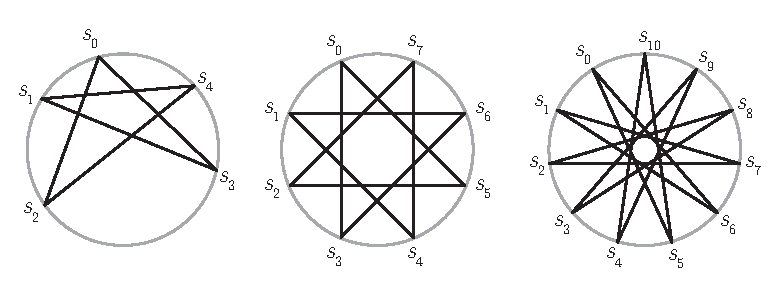
\includegraphics[scale=1]{starpolygons.eps}}
\caption{\small{Star polygons of type $\{5/2\}$, $\{8/3\}$ and $\{11/5\}$.}}\label{starpolygons}
\end{figure}

The main goal of this paper is to study $k$-triangulations as complexes of $k$-stars. Using this new tool, we get the first direct proof of property (i) (section \ref{sectioncomplexes}). Moreover, we obtain a simple description of flips, and consequently, an easy direct ({\it i.e.} non recursive) proof of (iii) (section \ref{sectionflips}). In section \ref{sectionflatinflat}, we present a new interpretation of (iv) as the flattening of a $k$-star. Then, we prove directly (ii), and we discuss the equality case (section \ref{sectionears}).

The second part of this paper deals with the combinatorics of the polygonal complex corresponding to a $k$-triangulaiton. In section \ref{sectionsurfaces}, we associate to a $k$-triangulation of an $n$-gon a decomposition of a surface $\mathcal{S}_{n,k}$ and we study the action of flips on this surface. In particular, we derive in section \ref{sectionregulardecomp} an application of $k$-triangulations to the construction of strongly regular decompositions of surfaces of high genus.

Finally, we discuss in section \ref{sectionopen} further topics that may be easier when using $k$-stars.




%%%%%%%%%%%%%%%%%%%%%%%%%%%%%%%%%%%%%%%%%%%%%%%%%%%%%%%%


\section{Notation}\label{sectionnotation}

Let $k$ and $n$ be two integers such that $k\ge 1$ and $n\ge 2k+1$.

Let $V_n$ be the \emph{set of vertices of an $n$-gon}, {\it i.e.} any set of points of the unit circle, labelled counterclockwise by the cyclic set $\mathbb{Z}_n$.
All throughout the paper, we will refer to the points in $V_n$ by their labels to simplify notation.
For $u,v,w\in V_n$, we will denote $u\cl v\cl w$ the cyclic order inherited from $\mathbb{Z}_n$.
For any $u,v\in V_n$, let $\llbracket u,v\rrbracket$ denote the \emph{cyclic interval} $\{w\in V_n\;|\; u\cle w\cle v\}$.
The intervals $\rrbracket u,v\llbracket$, $\llbracket u,v\llbracket$ and $\rrbracket u,v\rrbracket$ are defined similarly.
Let $|u-v|=\min(|\llbracket u, v\llbracket|,|\llbracket v, u\llbracket|)$ be the \emph{cyclic distance} between $u$ and $v$.

For $u\ne v\in V_n$, let $[u,v]$ denote the \emph{edge} connecting the vertices $u$ and $v$.
Let $E_n={V_n \choose 2}$ be the \emph{set of edges of the $n$-gon}.
Two edges $[u,v]$ and $[u',v']$ are said to be \emph{intersecting} when the open segments $]u,v[$ and $]u',v'[$ are intersecting.
For $\ell\in\mathbb{N}$, an \emph{$\ell$-crossing} is a set of $\ell$ mutually intersecting edges.
A \emph{$k$-triangulation} of the $n$-gon is a maximal $(k+1)$-crossing-free subset of $E_n$.

Obviously, an edge $[u,v]$ of $E_n$ can appear in a $(k+1)$-crossing only if $|u-v|>k$. We say that such an edge is \emph{$k$-relevant}. We say that an edge $[u,v]$ is a \emph{$k$-boundary} if $|u-v|=k$ and is \emph{$k$-irrelevant} if $|u-v|<k$.
Every $k$-triangulation of the $n$-gon contains all the $(k-1)n$ $k$-irrelevant edges and all the $n$ $k$-boundary edges of the $n$-gon and some $k$-relevant edges.

An \emph{angle} of a subset $E$ of $E_n$ is a pair of edges $\angle(u,v,w)=\{[u,v],[v,w]\}$ of $E$ such that $u\cl v\cl w$ and for all $t\in\rrbracket w,u\llbracket$, the edge $[v,t]$ is not in $E$. The vertex $v$ is the \emph{vertex} of $\angle(u,v,w)$. Any $t\in\rrbracket w,u\llbracket$ is said to be \emph{contained} in $\angle(u,v,w)$, and the edge $[v,t]$ is a \emph{bisector} of $\angle(u,v,w)$.
The bisectors of $E$ are the bisectors of all the angles of $E$.
An angle is said to be \emph{$k$-relevant} if its edges are either $k$-relevant or $k$-boundary edges.

Finally, observe that there are two natural cyclic orders on the vertices of a $k$-star $S$: the \emph{circle order}, defined as the cyclic order around the circle, and the \emph{star order}, defined as the cyclic order tracing the edges of $S$. More precisely, if $s_0,\ldots,s_{2k}$ are the vertices of $S$ cyclically ordered around the circle, we rename the vertices $r_i=s_{iq}$ to obtain the star order $r_0,\ldots,r_{2k}$.


%%%%%%%%%%%%%%%%%%%%%%%%%%%%%%%%%%%%%%%%%%%%%%%%%%%%%%%%


\section{Mutual positions of $k$-stars}\label{sectionstars}

In this section, we study the mutual positions of two $k$-stars $R$ and $S$ of a $(k+1)$-crossing-free subset $E$ of $E_n$.

\begin{lemma}\label{starangles}
Any angle of $S$ is an angle of $E$ and is $k$-relevant.
\end{lemma}

\begin{proof}
Let $V=\{s_j\;|\; j\in\mathbb{Z}_{2k+1}\}$ denote the vertices of $S$ in star order.
Suppose that $E$ contains an edge $[s_j,t]$ where $j\in\mathbb{Z}_{2k+1}$ and $t\in\rrbracket s_{j+1},s_{j-1}\llbracket$. Then the set of edges $$[s_{j+1},s_{j+2}],[s_{j+3},s_{j+4}],\ldots,[s_{j-2},s_{j-1}],[s_j,t]$$ forms a $(k+1)$-crossing. Thus $\angle(s_{j-1},s_j,s_{j+1})$ is an angle of $E$.

Since any edge of $S$ separates the other vertices of $S$ into two parts of size $k-1$ and $k$, it is at least a $k$-boundary. Consequently, the angle $\angle(s_{j-1},s_j,s_{j+1})$ is $k$-relevant.
\end{proof}

Note that this lemma implies that the knowledge of one angle $\angle(s_{j-1},s_j,s_{j+1})$ of $S$ permits the recovery of all the $k$-star $S$: the vertex $s_{j+2}$ is the unique vertex such that $\angle(s_j,s_{j+1},s_{j+2})$ is an angle of $E$ ({\it i.e.} the first neighbour of $s_{j+1}$ after $s_j$ when moving clockwise), and so on.
In particular, we get the following corollary.

\begin{corollary}
$R$ and $S$ can not share any angle.
\end{corollary}

Since the number of edges of a $k$-star is $2k+1$, this implies that $R$ and $S$ can not share more than $k$ edges. Note that they may share $k$ edges (for example, the two $k$-stars of the graph obtained from the complete graph on $2k+2$ vertices by omitting the diagonal $[0,k+1]$ share all the $k$  other diagonals).

\begin{corollary}
For any edge $[u,v]$ of $E$, the number $|\llbracket u,v\rrbracket\cap V|$ of vertices of $S$ between $u$ and $v$ and the number $|\llbracket v,u\rrbracket\cap V|$ of vertices of $S$ between $v$ and $u$ can not be equal.
\end{corollary}

\begin{proof}
Suppose that $S$ has the same number of vertices on both sides of an edge $f=[u,v]$. Since the number of vertices of $S$ is $2k+1$, one of the two vertices of $f$ is a vertex of $S$, say $u$. Then $v$ is contained in the angle of $S$ of vertex $u$, which implies that $f$ is not in $E$.
\end{proof}

If $|\llbracket u,v\rrbracket\cap V|>|\llbracket v,u\rrbracket\cap V|$, then we say that the $k$-star $S$ lies \emph{between} $u$ and $v$ (otherwise we say that $S$ lies between $v$ and $u$). 
The $k$-star $S$ is said to be contained in an angle $\angle(u,v,w)$ of $E$ if it lies between $v$ and $u$ and between $w$ and $v$.

\begin{lemma}
Let $\angle(u,v,w)$ be an angle of $E$ containing the $k$-star $S$. Then
\begin{enumerate}[(i)]
\item either $\angle(u,v,w)$ is an angle of $S$;
\item or $\angle(u,v,w)$ and $S$ have a common bisector (and $v$ is not a vertex of $S$).
\end{enumerate}
\end{lemma}

\begin{proof}
Suppose first that $v$ is a vertex of $S$. Let $\angle(x,v,y)$ denote the angle of $S$ of vertex $v$. Since $\angle(u,v,w)$ contains $S$, we have $w\cle y\cl x\cle u$. But since $\angle(u,v,w)$ is an angle, we have $x=u$ and $y=w$, so that $\angle(u,v,w)$ is an angle of $S$.

Suppose now that $v$ is not a vertex of $S$. Then there exists an angle $\angle(x,y,z)$ of $S$ containing $v$. If $y\in\rrbracket u,v\llbracket$, then $\rrbracket u,v\llbracket$ contains all the $k+1$ vertices of $S$ between $y$ and $z$, which is not possible (because $S$ lies between $v$ and $u$). If $y=u$, then $[u,v]$ is a bisector of $\angle(x,y,z)$, which contradicts lemma \ref{starangles}. Similarly, $y$ can not be in $\rrbracket v,w\rrbracket$. Consequently, $\angle(u,v,w)$ contains $y$, so that $[v,y]$ is a common bisector of $\angle(u,v,w)$ and $S$.
\end{proof}

\begin{theorem}\label{common bisector}
Every pair of $k$-stars contained in a $(k+1)$-crossing-free subset of $E_n$ have a unique common bisector.
\end{theorem}

\begin{proof}
Let $\{r_j\;|\; j\in\mathbb{Z}_{2k+1}\}$ denote the vertices of $R$ in star order. Note that for any $j\in\mathbb{Z}_{2k+1}$, if $S$ lies between $r_{j-1}$ and $r_j$, then it lies between $r_{j+1}$ and $r_j$. Since $2k+1$ is odd, this implies that there exists $j\in\mathbb{Z}_{2k+1}$ such that $S$ lies between $r_j$ and $r_{j-1}$ and between $r_{j+1}$ and $r_j$, {\it i.e.} in the angle $\angle(r_{j-1},r_j,r_{j+1})$.The previous lemma thus ensures the existence of a common bisector.

Suppose now that we have two common bisectors $e$ and $f$  of $R$ and $S$, and let $\{r_j\;|\; j\in\mathbb{Z}_{2k+1}\}$ and $\{s_j\;|\; j\in\mathbb{Z}_{2k+1}\}$ denote the vertices of $R$ and $S$ in star order such that $e=[r_0,s_0]$. Let $a,b\in\mathbb{Z}_{2k+1}$ such that $f=[r_a,s_b]$.
Note that certainly, $a\ne0$, $b\ne0$, and $a$ and $b$ have the same parity. By symmetry, we can assume that $a=2\alpha$, $b=2\beta$ with $1\le\beta\le\alpha\le k$. But then the set
$$\{[r_{2i},r_{2i+1}]\;|\; 0\le i\le \alpha-1\}\cup\{[s_{2j},s_{2j+1}]\;|\; \beta\le j\le k\}$$
forms a $(k+1+\alpha-\beta)$-crossing, and $k+1+\alpha-\beta\ge k+1$. This proves uniqueness.\end{proof}

\begin{figure}
\centerline{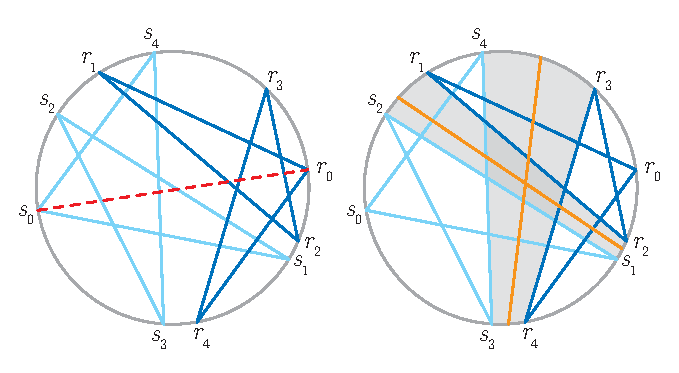
\includegraphics[scale=1]{combisector.eps}}
\caption{\small{The common bisector of two $2$-stars (left) and a $2$-crossing that crosses it (right).}}\label{combisector}
\end{figure}

In the following lemmas, $\{r_j\;|\; j\in\mathbb{Z}_{2k+1}\}$ and $\{s_j\;|\; j\in\mathbb{Z}_{2k+1}\}$ denote the vertices of $R$ and $S$, in star order, and such that $e=[r_0,s_0]$ is the common bisector of $R$ and $S$.

\begin{lemma}\label{paralleledges}
For every $1\le i\le k$, $r_{2i-1}\in\rrbracket r_0,s_{2i}\rrbracket$ and $s_{2i-1}\in\rrbracket s_0,r_{2i}\rrbracket$.
In particular, for every $i\in\mathbb{Z}_{2k+1}$ the edges $[r_i,r_{i+1}]$ and $[s_i,s_{i+1}]$ do not cross.
\end{lemma}

\begin{proof}
Suppose that there exists $1\le i\le k$ such that $r_{2i-1}\in\rrbracket s_{2i},s_0\llbracket$ or $s_{2i-1}\in\rrbracket r_{2i},r_0\llbracket$. Let $\gamma$ be the highest such integer, and assume for example that $r_{2\gamma-1}\in\rrbracket s_{2\gamma},s_0\llbracket$. Then the definition of $\gamma$ ensures that
$s_0\cl s_{2\gamma+1}\le r_{2\gamma}\cl r_{2\gamma-2}$
so that the set
$$\{[r_{2i},r_{2i+1}]\;|\; 0\le i\le\gamma-1\}\cup\{[s_{2j},s_{2j+1}]\;|\; \gamma\le j\le k\}$$
forms a $(k+1)$-crossing.
\end{proof}

The previous lemma can be read as saying that corresponding edges of $R$ and $S$ are parallel. It is easy to see that $k$ of these $2k+1$ pairs of parallel edges, the ones of the form $([r_{2i-1},r_{2i}],[s_{2i-1},s_{2i}])$, with $1\le i\le k$, separate $R$ from $S$. The next lemma says that any $k$-crossing that crosses the common bissector $e=[r_0,s_0]$ has one edge parallel to and between each such pair (see fig. \ref{combisector}).

\begin{lemma}\label{sandwich}
Let $F$ be a $k$-crossing of $E$ such that any of its edges crosses $e=[r_0,s_0]$. Let $f_1=[x_1,y_1],\ldots,f_k=[x_k,y_k]$ denote its edges such that $r_0\cl x_1\cl \ldots\cl x_k\cl s_0\cl y_1\cl \ldots\cl y_k\cl r_0$.
Then for any $1\le i\le k$, we have $x_i\in\llbracket r_{2k-2i+1},s_{2k-2i+2}\rrbracket$ and $y_i\in\llbracket s_{2k-2i+1},r_{2k-2i+2}\rrbracket$.
\end{lemma}

\begin{proof}
Suppose that there exists $1\le i\le k$ such that $r_0\cl x_i\cl r_{2k-2i+1}$ and let
$$\ell=\max\{1\le i\le k \;|\; r_0\cl x_i\cl r_{2k-2i+1}\}.$$
If $\ell=k$, then the set $\{e_1,\ldots,e_k,[r_0,r_1]\}$ is a $(k+1)$-crossing of $T$, thus we assume that $\ell<k$. In order for $$\{e_1,\ldots,e_\ell\}\cup\{[r_0,r_1],\ldots,[r_{2k-2\ell},r_{2k-2\ell+1}]\}$$ not to be a $(k+1)$-crossing, we have $r_{2k-2\ell}\cle y_\ell\cl r_0$, so that $r_{2k-2\ell}\cl y_{\ell+1}\cl r_0$. But the definition of $\ell$ implies that $r_{2k-2\ell+1}\cl r_{2k-2\ell-1}\cle x_{\ell+1}\cl s_0$, so that
the set $$\{[r_{2k-2\ell},r_{2k-2\ell+1}],\ldots,[r_{2k-2},r_{2k-1}],[r_{2k},r_0]\}\cup\{e_{\ell+1},\ldots,e_k\}$$ is a $(k+1)$-crossing of $T$.

By symmetry, the lemma is proved.
\end{proof}

The following lemma is at the heart of the concept of flips to be studied further in section \ref{sectionflips}.

\begin{lemma}\label{commonedge}
Let $f$ be a common edge of $R$ and $S$. Then
\begin{enumerate}[(i)]
\item there exists $1\le i\le k$ such that $f=[r_{2i-1},r_{2i}]=[s_{2i},s_{2i-1}]$;
\item $E\triangle\{e,f\}$ is a $(k+1)$-crossing-free subset of $E_n$;
\item the vertices $$s_0,\ldots,s_{2i-2},s_{2i-1}=r_{2i},r_{2i+1},\ldots,r_{2k},r_0$$
(resp. $r_0,\ldots,r_{2i-2},r_{2i-1}=s_{2i},s_{2i+1},\ldots,s_{2k},s_0$) are the vertices of a $k$-star $X$ (resp. $Y$) of $E\triangle\{e,f\}$, in star order;
\item $X$ and $Y$ share the edge $e$ and their common bisector is $f$.
\end{enumerate}
\end{lemma}

\begin{figure}
\centerline{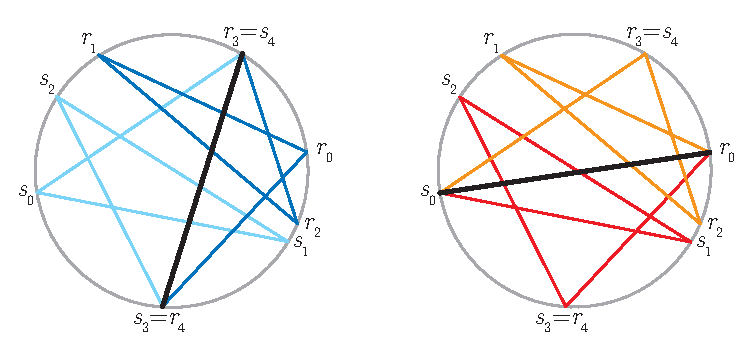
\includegraphics[scale=1]{flip.eps}}
\caption{\small{The flip of an edge.}}\label{flip}
\end{figure}

\begin{proof}
Let $u$ and $v$ denote the vertices of $f$.
Lemma \ref{paralleledges} ensures that $\{r_0,s_0\}\cap\{u,v\}=\emptyset$ so that we can assume $r_0\cl u\cl s_0\cl v\cl r_0$. Consequently, there exists $1\le i,j\le k$ such that $u=r_{2i-1}=s_{2j}$ and $v=r_{2i}=s_{2j-1}$. Suppose that $i>j$. Then according to  lemma \ref{paralleledges}, we have $r_0\cl r_{2i-1}\cle s_{2i}\cl s_{2j}=r_{2i-1}$ which is impossible. We obtain that $i=j$ and $f=[r_{2i-1},r_{2i}]=[s_{2i},s_{2i-1}]$.

Lemma \ref{sandwich} then proves that any $k$-crossing of $T$ that prevent $e$ being in $T$ contains $f$, so that $T\triangle\{e,f\}$ does not contain any $(k+1)$-crossing.

Moreover, for any $1\le j\le p$, the number of vertices of the set $\{s_0,\ldots,s_{2i-2},r_{2i},\ldots,r_{2k},r_0\}$ between $s_{2j-2}$ and $s_{2j-1}$ (resp. $r_{2j}$ and $r_{2j+1}$, resp. $r_0$ and $s_0$) is obviously $k-1$. This implies that the vertices $s_0,\ldots,s_{2i-2},r_{2i},\ldots,r_{2k},r_0$ are in star order. The point (iii) thus follows from the fact that any edge connecting two consecutive points of this list is in $E\triangle\{e,f\}$.

The edge $e$ is clearly common to $X$ and $Y$. The edge $f$ is a bisector of both angles $\angle(r_{2i-2},r_{2j-1},s_{2i+1})$ and $\angle(s_{2i-2},s_{2j-1},r_{2i+1})$, so that it is the common bisector of $X$ and $Y$.
\end{proof}



%%%%%%%%%%%%%%%%%%%%%%%%%%%%%%%%%%%%%%%%%%%%%%%%%%%%%%%%%

\section{$k$-triangulations as complexes of $k$-stars}\label{sectioncomplexes}

In this section, $T$ is a $k$-triangulation of the $n$-gon, {\it i.e.} a maximal $(k+1)$-crossing-free subset of $E_n$.

\begin{theorem}\label{angle}
Any $k$-relevant angle of a $k$-triangulation $T$ belongs to a unique $k$-star of $T$.
\end{theorem}


\begin{proof}
In this proof, we need the following definition (see fig. \ref{farther}): let $\angle(u,v,w)$ be a $k$-relevant angle of $T$ and let $e$ and $f$ be two edges of $T$ that \emph{intersect} $\angle(u,v,w)$ ({\it i.e.} that intersect both $[u,v]$ and $[v,w]$). If $a,b,c$ and $d$ denote their vertices such that $u\cl a\cl v\cl b\cl w$ and $u\cl c\cl v\cl d\cl w$, then we say that $e=[a,b]$ is \emph{$v$-farther} than $f=[c,d]$ if $u\cl a\cle c\cl v\cl d\cle b\cl w$. Let $E$ and $F$ be two $(k-1)$-crossings that \emph{intersect} $\angle(u,v,w)$. Let their edges be labelled $e_1=[a_1,b_1],e_2=[a_2,b_2],\ldots,e_{k-1}=[a_{k-1},b_{k-1}]$ and $f_1=[c_1,d_1],f_2=[c_2,d_2],\ldots,f_{k-1}=[c_{k-1},d_{k-1}]$ such that $u\cl a_1\cl a_2\cl \ldots\cl a_{k-1}\cl v\cl b_1\cl b_2\cl \ldots\cl b_{k-1}\cl w$ and $u\cl c_1\cl c_2\cl \ldots\cl c_{k-1}\cl v\cl d_1\cl d_2\cl \ldots\cl d_{k-1}\cl w$. Then we say that $E$ is \emph{$v$-farther} than $F$ if $e_i$ is $v$-farther than $f_i$ for every $1\le i\le k-1$. We say that $E$ is \emph{$v$-maximal} if it does not exist any $(k-1)$-crossing intersecting $\angle(u,v,w)$ and $v$-farther than $E$

\begin{figure}
\centerline{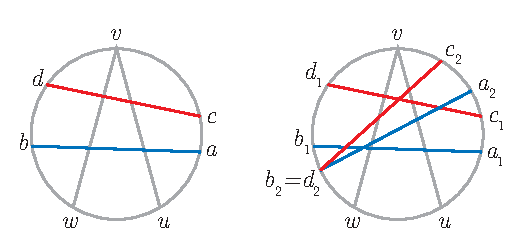
\includegraphics[scale=1]{farther.eps}}
\caption{\small{$[a,b]$ is $v$-farther than $[c,d]$ (left) and $\{[a_i,b_i]\}$ is $v$-farther than $\{[c_i,d_i]\}$ (right).}}\label{farther}
\end{figure}

Let $\angle(u,v,w)$ be a $k$-relevant angle of $T$. 
If the edge $[u,v+1]$ is in $T$, then the angle $\angle(v+1,u,v)$ is a $k$-relevant angle of $T$ and, if it is contained in a $k$-star $S$ of $T$, then so is $\angle(u,v,w)$. Moreover, if $n>2k+1$ ($n=2k+1$ is a trivial case), $T$ can not contain all the edges $\{[u+i,v+i]\;|\; i=0\ldots n-1\}$ and $\{[u+i,v+i+1]\;|\; i=0\ldots n-1\}$. Consequently, we can assume that $[u,v+1]$ is not in $T$.

Thus we have a $k$-crossing $E$ of the form $e_1=[a_1,b_1],\ldots,e_k=[a_k,b_k]$ with $u\cl a_1\cl \ldots\cl a_k\cl v+1$ and $v+1\cl b_1\cl \ldots\cl b_k\cl u$. Since $[u,v]\in T$, $a_k=v$ and since $\angle(u,v,w)$ is an angle, $v+1\cl b_k\cle w$. Consequently, $\{e_1,\ldots,e_{k-1}\}$ forms a $(k-1)$-crossing intersecting $\angle(u,v,w)$ and we can assume that it is $v$-maximal (see fig. \ref{twosteps} (a)). We will prove that the edges $[u,b_1], [a_1,b_2],\ldots, [a_{k-2},b_{k-1}],[a_{k-1},w]$ are in $T$ such that the points $u$, $a_1,\ldots,a_{k-1}$, $v$, $b_1,\ldots,b_{k-1}$, $w$ are the vertices of a $k$-star of $T$ containing the angle $\angle(u,v,w)$. To get this result, we use two steps: first we prove that $\angle(a_1,b_1,u)$ is an angle of $T$, and then we prove that the edges $e_2,\ldots,e_{k-1},[v,w]$ form a $(k-1)$-crossing intersecting $\angle(a_1,b_1,u)$ and $b_1$-maximal (so that we can reiterate the argument).

\medskip
\noindent\textsc{First step.}  (see fig. \ref{twosteps} (b))

Suppose that $[u,b_1]$ is not in $T$. Thus we have a $k$-crossing $F$ that prevents the edge $[u,b_1]$. Let $f_1=[c_1,d_1],\ldots,f_k=[c_k,d_k]$ denote its edges with $u\cl c_1\cl \ldots\cl c_k\cl b_1$ and $b_1\cl d_1\cl \ldots\cl d_k\cl u$.

Note first that $v\cl d_k\cle w$. Indeed, if it is not the case, then $d_k\in\rrbracket w,u\llbracket$ and $c_k\ne v$, because $\angle(u,v,w)$ is an angle. Thus either $c_k\in\rrbracket u,v\llbracket$ and  then $F\cup\{[u,v]\}$ forms a $(k+1)$-crossing, or $c_k\in\rrbracket v,b_1\llbracket$ and  then $E\cup\{[c_k,d_k]\}$ forms a $(k+1)$-crossing. Consequently, we have $b_1\cl d_1\cl \ldots\cl d_{k-1}\cl w$.

Let $\ell=\max\{1\le i\le {k-1}\;|\; b_i\cl d_i\cl w\}$. Then for any $1\le i\le\ell$, since $\{e_1,\ldots,e_i\}\cup\{f_i,\ldots,f_k\}$ does not form a $(k+1)$-crossing, we have $u\cl c_i\cle a_i$. Thus for any $1\le i\le\ell$, $u\cl c_i\cle a_i\cl v\cl b_i\cl d_i\cl w$, so that $f_i$ is $v$-farther than $e_i$. Furthermore, we have $u\cl c_1\cl \ldots\cl c_\ell\cl a_{\ell+1}\cl\ldots\cl a_{k-1}\cl v\cl d_1\cl\ldots\cl d_\ell\cl b_{\ell+1}\cl \ldots\cl b_{k-1}\cl w$. Consequently, we get a $(k-1)$-crossing $\{f_1,\ldots,f_\ell,e_{\ell+1},\ldots,e_{k-1}\}$ which is $v$-farther than $\{e_1,\ldots,e_{k-1}\}$; this contradicts the definition of $\{e_1,\ldots,e_{k-1}\}$. Thus we obtain $[u,b_1]\in T$.

Suppose now that $\angle(a_1,b_1,u)$ is not an angle of $T$ then there exists $a_0\in \rrbracket u,a_1\llbracket$ such that $[b_1,a_0]\in T$. But then the $(k-1)$-crossing $\{[a_0,b_1],e_2,\ldots,e_{k-1}\}$ is $v$-farther than $\{e_1,\ldots,e_{k-1}\}$, so that $\angle(a_1,b_1,u)$ is an angle of $T$.
\begin{figure}

\centerline{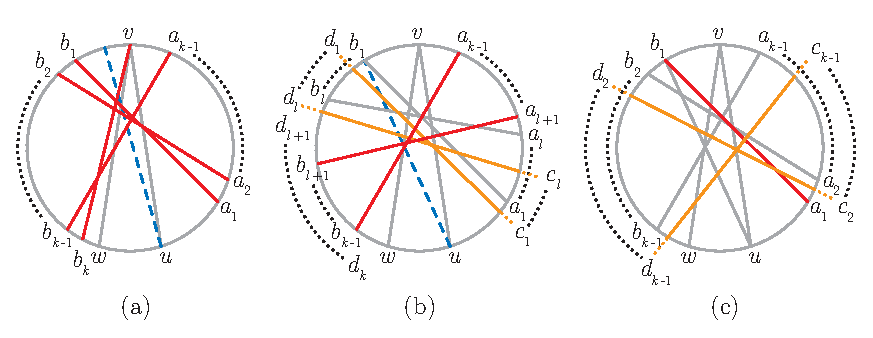
\includegraphics[scale=1]{twosteps.eps}}
\caption{\small{(a) the $k$-crossing $E$; (b) First step: $[u,b_1]\in T$; (c) Second step: $\{e_2,\ldots,e_{k-1},[v,w]\}$ is $b_1$-maximal.}}\label{twosteps}
\end{figure}

\medskip
\noindent\textsc{Second step.} (see fig. \ref{twosteps} (c))

Let $F$ be a $(k-1)$-crossing intersecting $\angle(a_1,b_1,u)$ and $b_1$-farther than the $(k-1)$-crossing $\{e_2,\ldots,e_{k-1},[v,w]\}$. Let $f_2=[c_2,d_2],\ldots,f_k=[c_k,d_k]$ denote its edges such that $a_1\cl c_2\cl \ldots\cl c_k\cl b_1\cl d_2\cl \ldots\cl d_k\cl u$. 

Note first that $b_k\cle d_k\cle w$. Indeed, if it is not the case, then $d_k\in\rrbracket w,u\llbracket$ and $c_k\ne v$, because $\angle(u,v,w)$ is an angle. Thus either $c_k\in\rrbracket a_1,v\llbracket$ and  then $F\cup\{[u,v],e_1\}$ forms a $(k+1)$-crossing, or $c_k\in\rrbracket v,b_1\llbracket$ and  then $E\cup\{[c_k,d_k]\}$ forms a $(k+1)$-crossing. Consequently, we have $b_1\cl d_2\cl\ldots\cl d_{k-1}\cl w$.

Furthermore, for any $2\le i\le k-1$, $f_i$ is $\angle(a_1,b_1,u)$-farther than $e_i$, so that $a_1\cl c_i\cle a_i\cl b_1\cl b_i\cle d_i\cl u$. In particular, $a_1\cl c_{k-1}\cle a_{k-1}\cl v$ and we get $u\cl a_1\cl c_2\cl\ldots\cl c_{k-1}\cl v\cl b_1\cl d_2\cl \ldots\cl d_{k-1}\cl w$. Consequently, the $(k-1)$-crossing $\{e_1,f_2,\ldots,f_{k-1}\}$ is $v$-farther than $\{e_1,\ldots,e_{k-1}\}$, which is a contradiction.
\end{proof}

The following easy corollary of theorem \ref{angle} justifies the title of this paper.

\begin{corollary}\label{incidences}
Let $e$ be an edge of $T$. Then
\begin{enumerate}[(i)]
\item if $e$ is a $k$-relevant edge, then it belongs to exactly two $k$-stars of $T$ (one on each side);
\item if $e$ is a $k$-boundary edge, then it belongs to exactly one $k$-star of $T$ (on its inner side); \item if $e$ is a $k$-irrelevant edge, then it does not belong to any $k$-star of $T$.
\end{enumerate}
\end{corollary}

\begin{corollary}\label{findingstars}
\begin{enumerate}
\item For any $k$-star $S$ of $T$ and for any vertex $r$ not in $S$ there is a unique $k$-star $R$ of $T$ such that $r$ is a vertex of the common bisector of $R$ and $S$.
\item Any $k$-relevant edge which is not in $T$ is the common bisector of a unique pair of $k$-stars of $T$.
\end{enumerate}
\end{corollary}

\begin{proof}
Let $\angle(u,s,v)$ be the unique angle of $S$ which contains $r$. Let $\angle(x,r,y)$ be the unique angle of $T$ of vertex $r$ which contains $s$. According to theorem \ref{angle}, the angle $\angle(x,r,y)$ belongs to a unique $k$-star $R$. The common bisector of $R$ and $S$ is $[r,s]$ and $R$ is the only such $k$-star of $T$.

Let $e=[r,s]$ be a $k$-relevant edge, not in $T$. Let $\angle(x,r,y)$ (resp. $\angle(u,s,v)$) denote the unique angle of $T$ of vertex $r$ (resp. $s$) which contains $s$ (resp. $r$). According to theorem \ref{angle}, the angle $\angle(x,r,y)$ (resp. $\angle(u,s,v)$) belongs to a unique $k$-star $R$ (resp. $S$). The common bisector of $R$ and $S$ is $[r,s]$ and $(R,S)$ is the only such couple of $k$-stars of $T$.
\end{proof}

Observe that parts (1) and (2) of this lemma give bijections from 
\begin{enumerate}
\item ``vertices not used in a $k$-star $S$ of $T$" and ``$k$-stars of $T$ distinct from $S$";
\item ``$k$-relevant edges not used in $T$" and ``pairs of $k$-stars of $T$".
\end{enumerate}
From any of these bijections, and using corollary \ref{incidences} for double counting, it is easy to derive the number of $k$-stars and $k$-relevant edges in $T$:

\begin{corollary}\label{starsenumeration}
\begin{enumerate}
\item Any $k$-triangulation of the $n$-gon contains exactly $n-2k$ $k$-stars, $k(n-2k-1)$ $k$-relevant edges and $k(2n-2k-1)$ edges.
\item The $k$-triangulations of the $n$-gon are exactly the $(k+1)$-crossing free subsets of $E_n$ of cardinality $k(2n-2k-1)$.
\end{enumerate}
\end{corollary}




%%%%%%%%%%%%%%%%%%%%%%%%%%%%%%%%%%%%%%%%%%%%%%%%%%%%%%%%%


\section{The graph of flips}\label{sectionflips}

Let $T$ be a $k$-triangulation of the $n$-gon, let $f$ be a $k$-relevant edge of $T$, let $R$ and $S$ be the two $k$-stars of $T$ containing $f$ (corollary \ref{incidences}), and let $e$ be the common bisector of $R$ and $S$. Remind that we proved (lemma \ref{commonedge}) that $T\triangle\{e,f\}$ is a $(k+1)$-crossing-free subset of $E_n$. Observe moreover that $T\triangle\{e,f\}$ is maximal: this follows from corollary \ref{starsenumeration}, but also from the fact that if $T\triangle\{e,f\}$ is properly contained in a $k$-triangulation $\widetilde{T}$, then $\widetilde{T}\triangle\{e,f\}$ is $(k+1)$-crossing-free and properly contains $T$. Thus $T\triangle\{e,f\}$ is a $k$-triangulation of the $n$-gon.

\begin{lemma}\label{flip}
$T$ and $T\triangle\{e,f\}$ are the only two $k$-triangulations of the $n$-gon contaning $T\setminus\{f\}$.
\end{lemma}

\begin{proof}
Let $e'$ be any edge of $E_n\setminus T$ distinct from $e$. Let $R'$ and $S'$ be the two $k$-stars with common bisector $e'$ (lemma \ref{findingstars} (2)). We can assume that $R'$ does not contain $f$ and then $R'\cup\{e'\}$ is contained in $T\triangle\{e',f\}$ and forms a $(k+1)$-crossing.
\end{proof}

We say that we obtain the $k$-triangulation $T\triangle\{e,f\}$ from the $k$-triangulation $T$ by \emph{flipping} the edge $f$. The $k$-triangulations $T$ and $T\triangle\{e,f\}$ are said to be \emph{flip-neighbours}. The added edge $e$ is denoted by $e(T,f)$.

Let $G_{n,k}$ be the graph of flip-neighbours on the set of $k$-triangulations of the $n$-gon, {\it i.e.} the graph whose vertices are the $k$-triangulations of the $n$-gon and whose edges are the pairs of flip-neighbour $k$-triangulations.

In this section, we prove the connexity of this graph.

\medskip
Note that $e$ and $f$ necessarily cross.
In particular, if $e=[\alpha,\beta]$ and $f=[\gamma,\delta]$, with $0\cle\alpha\cl\beta\cle n-1$ and $0\cle\gamma\cl\delta\cle n-1$, then
\begin{itemize}
\item either $0\cle\alpha\cl\gamma\cl\beta\cl\delta\cle n-1$ and the flip is said to be \emph{slope-decreasing},
\item or $0\cle\gamma\cl\alpha\cl\delta\cl\beta\cle n-1$ and the flip is said to be \emph{slope-increasing}.
\end{itemize}
We define a partial order on the set of $k$-triangulations of the $n$-gon as follows: if $T$ and $T'$ are two $k$-triangulations of the $n$-gon, $T<T'$ if and only if there exists a sequence of slope-increasing flips from $T$ to $T'$ (if and only if there exists a sequence of slope-decreasing flips from $T'$ to $T$).

Let $T_{n,k}^{\min}$ be the $k$-triangulation of the $n$-gon whose set of $k$-relevant edges is $\{[i,j]\;|\;i\in\llbracket 0,k-1\rrbracket\;\mathrm{and}\;j\in\llbracket i+k,i-k\rrbracket\}$ (see fig. \ref{min}).

\begin{figure}
\centerline{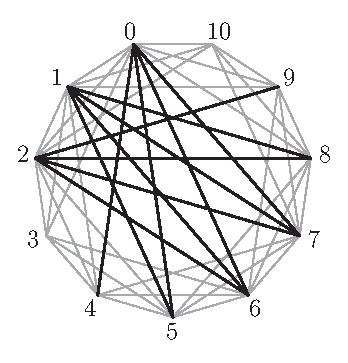
\includegraphics[scale=1]{min.eps}}
\caption{\small{The triangulation $T_{11,3}^{\min}$.}}\label{min}
\end{figure}

\begin{lemma}\label{connexity}
For any $k$-triangulation of the $n$-gon $T\ne T_{n,k}^{\min}$, there exists a $k$-relevant edge $f\in T\setminus T_{n,k}^{\min}$ such that $e(T,f)\in T_{n,k}^{\min}\setminus T$.

In particular, $T_{n,k}^{\min}$ is the least element of the set of $k$-triangulations of the $n$-gon partially ordered by $<$.
\end{lemma}

\begin{proof}
Since the second point is an immediate corollary of the first one, we only have to prove the first point.

Let $T$ be a $k$-triangulation of the $n$-gon distinct from $T_{n,k}^{min}$. Let
$$\ell=\max\{k\le i\le n-k+1\;|\;\{[0,i],[1,i+1],\ldots,[k-1,i+k-1]\}\nsubseteq T\},$$
which exists because $T\ne T_{n,k}^{min}$.

Let $0\le j\le k-1$ such that the edge $[j,\ell+j]$ is not in $T$. Let $\{[x_1,y_1],\ldots,[x_k,y_k]\}$ denote a $k$-crossing that prevent $[j,\ell+j]$ to be in $T$, with the convention that
\begin{enumerate}[(i)]
\item $x_1\cl \ldots\cl x_k\cl y_1\cl \ldots\cl y_k$,
\item if $j>0$, then $j\in\rrbracket x_j,x_{j+1}\llbracket$ and $\ell+j\in\rrbracket y_j,y_{j+1}\llbracket$,
\item if $j=0$, then $0\in\rrbracket y_k,x_1\llbracket$ and $\ell+j\in\rrbracket x_k,y_1\llbracket$.
\end{enumerate}
With this convention, we are sure that $x_k\in\llbracket k,\ell-1\rrbracket$ and $y_k\in\llbracket \ell+k,n-1\rrbracket$. If $y_k\in \rrbracket \ell+k,n-1\rrbracket$, then the set
$$\{[0,\ell],\ldots,[k-1,\ell+k],[x_k,y_k]\}$$
is a $(k+1)$-crossing of $T$. Thus $y_k=\ell+k$, and there exists an edge $[x_k,\ell+k]$ with $x_k\in\llbracket k,\ell-1\rrbracket$.

Now let $m=\min\{k\le i\le \ell-1\;|\; [i,\ell+k]\in T\}$. Let $f$ be the edge $[m,\ell+k]$, let $S$ be the $k$-star containing the angle $\angle(m,\ell+k,k-1)$ and let $R$ be the other $k$-star containing $f$. Let $s_0, \ldots,s_{k-2},s_{k-1}=k-1,s_k=m,s_{k+1},\ldots,s_{2k-1},s_{2k}=\ell+k$ denote the vertices of the $k$-star $S$ in circle order. Then $s_0\in\llbracket \ell+k+1, 0\rrbracket$, and the only way not to get a $(k+1)$-crossing is to have $s_0=0$. This implies that $s_j=j$ for all $0\le j\le k-1$. 

Let $e=e(T,f)$ be the common bisector of $R$ and $S$ and $s$ denote its vertex in $S$. Since $f=[m,\ell+k]=[s_k,s_{2k}]$ is a common edge of $R$ and $S$, it is obvious that $s\notin\{s_k,s_{2k}\}$. Moreover, since for any $0\le j\le k-1$ the interval $\rrbracket s_j,s_{j+1}\llbracket$ is empty, $s\notin\{s_{k+1},s_{k+2},\ldots,s_{2k-1}\}$. Consequently, $s\in\{s_0,\ldots,s_{k-1}\}=\llbracket 0,k-1\rrbracket$ and $e\in T_{n,k}^{\min}\setminus T$.
\end{proof}

Obviously, we get symetric results with the $k$-triangulation $T_{n,k}^{\max}$ whose set of $k$-relevant edges is $\{[i,j]\;|\;i\in\llbracket n-k,n-1\rrbracket\;\mathrm{and}\;j\in\llbracket i+k,i-k\rrbracket\}$.

\begin{corollary}
The graph $G_{n,k}$ is connected, regular of degree $k(n-2k-1)$, and its diameter is at most $2k(n-2k-1)$.
\end{corollary}

\begin{proof}
Let $T$ be a $k$-triangulation of the $n$-gon. The regularity follows from the fact that any of the $k(n-2k-1)$ $k$-relevant edges of $T$ can be flipped. Moreover, the previous lemma ensures that there exists a sequence of at most $k(n-2k-1)$ slope-decreasing flips from $T$ to $T_{n,k}^{\min}$. Thus any pair of $k$-triangulations is linked by a path of lenght at most $2k(n-2k-1)$ passing through $T_{n,k}^{\min}$.
\end{proof}

Obviously we would obtain the same result with any rotation of the labelling of $V_n$. In particular, for any pair $\{T,T'\}$ of $k$-triangulations, we can choose the intermediate $k$-triangulation $T''$ for our path among any rotation of $T_{n,k}^{\min}$. Consequently, there exists a path linking $T$ and $T'$ of length smaller than the average of $|T\triangle T''|+|T''\triangle T'|$ (for $T''$ among the rotations of $T_{n,k}^{\min}$). As proved in \cite{n-gdfcp-00}, the diameter upper bound can thus be improved to be $2kn-(8k^2+2k)$ when $n>8k^3+4k^2$.

Note that even if the improvement is asymptotically not relevant, for the case $k=1$, the improved bound of $2n-10$ is actually the exact diameter of the associahedron \cite{stt-rdthg-88}. For $k>1$, we only have the following lower bound:

\begin{lemma}\label{diamin}
If $n\ge 4k$, then the diameter of $G_{n,k}$ is at least $k(n-2k-1)$.
\end{lemma}

\begin{proof}
We only have to find two $k$-triangulations of the $n$-gon with no $k$-relevant edges in common. Let $Z$ be the subset of $k$-relevant edges of $E_n$ defined by
\begin{eqnarray*}
Z & = & \left\{[q-1,-q-k]\;|\; 1\le q\le \lfloor n/2-k\rfloor\right\}\\
&&\cup\left\{[q,-q-k]\;|\; 1\le q\le \lfloor (n-1)/2-k\rfloor\right\}.
\end{eqnarray*}
We say that $Z$ is a \emph{$k$-zigzag} of $E_n$ (see fig. \ref{zigzags}). Let $\rho$ be the rotation $t\mapsto t+1$. Observe that since $n\ge 4k$, the $2k$ $k$-zigzags $Z,\rho(Z),\ldots,\rho^{2k-1}(Z)$ are disjoint. Moreover,
\begin{enumerate}[(i)]
\item there is no $2$-crossing in a $k$-zigzag, so that there is no $(k+1)$-crossing in the union of $k$ $k$-zigzags;
\item a $k$-zigzag contains $n-2k-1$ $k$-relevant edges, so that the disjoint union of $k$ $k$-zigzags contains $k(n-2k-1)$ $k$-relevant edges.
\end{enumerate}
According to corollary \ref{starsenumeration}, this proves that the disjoint union of $k$ $k$-zigzag is the set of $k$-relevant edges of a $k$-triangulation. Thus, we obtain the two $k$-triangulations we were looking for with the sets of $k$-relevant edges $\bigcup_{i=0}^{k-1} \rho^i(Z)$ and $\bigcup_{i=k}^{2k-1} \rho^i(Z)$.
\begin{figure}
\centerline{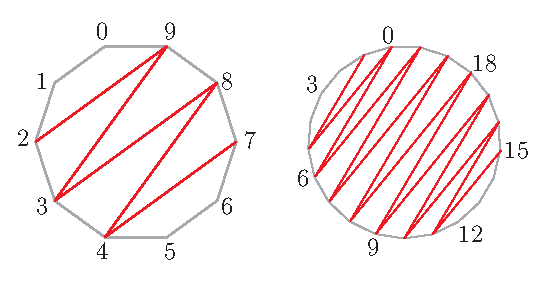
\includegraphics[scale=1]{zigzags.eps}}
\caption{\small{Examples of $k$-zigzags of $E_n$ for $(k,n)=(2,10)$ and $(3,21)$.}}\label{zigzags}
\end{figure}
\end{proof}

Finally, observe that lemma \ref{connexity} gives another proof of the number of edges (and consequently of $k$-stars) in a $k$-triangulation of the $n$-gon. This method is the one that is used in \cite{n-gdfcp-00} and \cite{dkm-lahp-02}.



%%%%%%%%%%%%%%%%%%%%%%%%%%%%%%%%%%%%%%%%%%%%%%%%%%%%%%%%%


\section{Flattening a $k$-star, inflating a $k$-crossing}\label{sectionflatinflat}

The goal of this section is to describe in terms of $k$-stars an operation that connects $k$-triangulations of $n$ and of $n+1$ vertices. This operation, already present in \cite{j-gt-03}, in \cite{n-gdfcp-00}, and when $k=2$ in \cite{e-btdp-06}, is useful for recursive arguments and it was a step in all previous proof of the flipability of a $k$-relevant edge.


\medskip
Let $T$ be a $k$-triangulation of the $(n+1)$-gon, and $e=[s_0,s_0+k]$ be a $k$-boundary edge of $T$.
Let $s_0,s_1=s_0+1,\ldots,s_k=s_0+k,s_{k+1},\ldots,s_{2k}$ be the vertices of the unique $k$-star of $T$ containing $e$, in the circle order.

We call \emph{flattening} of $e$ in $T$ the set of edges $\underline{T}_e$ whose underlying set of points is the set $V_{n+1}\smallsetminus\{s_0\}$ and which is contructed from $T$ as follows (see fig. \ref{flatinfl}):
\begin{enumerate}[(i)]
\item for any edge of $T$ whose vertices are not in $\{s_0,\ldots,s_k\}$ just copy the edge;
\item forget all the edges $[s_0,s_i]$, for $1\le i\le k$;
\item replace any edge of form $[s_i,t]$ with $0\le i\le k$, and $s+k+1\cle t \cle s_{k+i}$ (resp. $s_{k+i+1}\cle t\cle s-1$) by the edge $[s_i,t]$ (resp. $[s_{i+1},t]$).
\end{enumerate}

\begin{figure}
\centerline{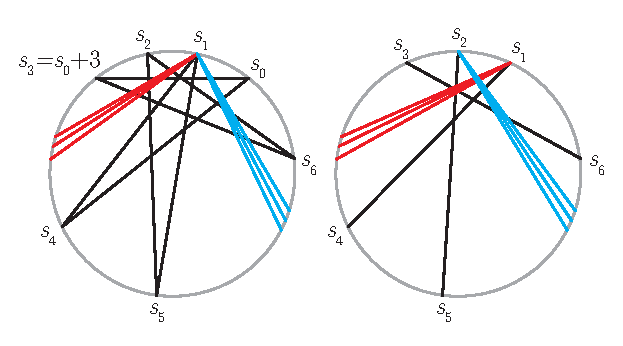
\includegraphics[scale=1]{flatinfl.eps}}
\caption{\small{Flattening a $3$-boundary edge - inflating a $3$-crossing.}}\label{flatinfl}
\end{figure}

\medskip
We want to prove that $\underline{T}_e$ is a $k$-triangulation of the $n$-gon. Observe first that
\begin{enumerate}
\item If $f$ is a $k$-relevant edge of $\underline{T}_e$, then
\begin{enumerate}[(i)]
\item either $f$ is of form $[s_i,s_{k+i}]$, for some $1\le i\le k$, and it arise from two edges $f'=[s_{i-1},s_{k+i}]$ and $f''=[s_i,s_{k+i}]$ of the initial triangulation $T$;
\item or $f$ is not of the previous form, and it arise from a unique $k$-relevant edge $f'$ of $T$.
\end{enumerate}

\item If $f$ and $g$ are two $k$-relevant edges of $\underline{T}_e$ arising from $f'$ and $g'$ respectively, then
\begin{enumerate}[(i)]
\item if $f$ and $g$ do not cross, then $f'$ and $g'$ do not cross; 
\item if $f$ and $g$ do cross, then $f'$ and $g'$ do cross, except if there exists $i$ in $\{1,\ldots,k\}$, and $u,v$ two vertices such that $s+k\cl u\cle s_{i+k}\cl s_{i+k+1}\cle v\cl s$ and $f=[r_i,u]$, $g=[r_{i+1},v]$, $f'=[s_i,u]$ and $g'=[s_i,v]$. Such a configuration is said to be a \emph{hidden configuration}.
\end{enumerate}
\end{enumerate}

It is easy to derive from this that $|\underline{T}_e|=|T|-2k=k(2n-2k-1)$ and that any subset of $E_n$ that properly contains $\underline{T}_e$ contains a $(k+1)$-crossing. However, observe that it is not sufficient to prove that $\underline{T}_e$ is a $k$-triangulation. Thus we have to prove that $\underline{T}_e$ is $(k+1)$-crossing-free. Note that it will provides a third proof (which this time is recursive) of the number of edges of a $k$-triangulation of the $n$-gon.

\begin{lemma}
The set $\underline{T}_e$ is $(k+1)$-crossing-free.
\end{lemma}

\begin{proof}
Let $F$ be a $(k+1)$-crossing of $\underline{T}_e$. We denote $f_1=[x_1,y_1],\ldots,f_{k+1}=[x_{k+1},y_{k+1}]$ the edges of $F$ ordered such that $x_1\cl x_2\cl\ldots\cl x_{k+1}\cl y_1\cl y_2\cl \ldots\cl y_{k+1}$. Let $f'_1=[x'_1,y'_1],\ldots,f'_{k+1}=[x'_{k+1},y'_{k+1}]$ denote $k$ edges of $T$ that give the edges $f_1,\ldots,f_{k+1}$ respectively.

It is clear that if there exists no $1\le i\le k+1$ such that $(f_i,f_{i+1},f'_i,f'_{i+1})$ form a hidden configuration, then the edges $f'_1,\ldots,f'_{k+1}$ form a $(k+1)$-crossing of $T$, which is impossible. Thus we can suppose that the number of hidden configurations in the set $\{(f_i,f_{i+1},f'_i,f'_{i+1})\;|\; 1\le i\le k+1\}$ is at least $1$. We will find a new $(k+1)$-crossing $G$ of $\underline{T}_e$ arising from a set $G'$ of edges of $T$ such that the number of hidden configurations in the set $\{(g_i,g_{i+1},g'_i,g'_{i+1})\;|\; 1\le i\le k+1\}$ is strictly less than in $\{(f_i,f_{i+1},f'_i,f'_{i+1})\;|\; 1\le i\le k+1\}$.

Let $i$ in $\{1,\ldots,k+1\}$ be such that $(f_i,f_{i+1},f'_i,f'_{i+1})$ is a hidden configuration. We can suppose that $x_i=s_i$ and $x_{i+1}=s_{i+1}$ (if this is not the case, we renumber the edges of $F$ such that this be true). Thus we know that $y_i\cle s_{i+k}\cl s_{i+k+1}\cle y_{i+1}$. Let $p$ denote the first integer before $i$ such that $x_p \ne s_p$ or $s_{p+k}\cl y_p$, and $q$ denote the first integer after $i+1$ such that $x_q \ne s_q$ or $y_q\cl s_{q+k}$.

Let $G$ be the set of $k+1$ edges of $\underline{T}_e$ deduced from $F$ as follows:
\begin{itemize}
\item for all $p<i<q$, let $g_i$ be $[s_i,s_{i+k}]$,
\item for all $q\le i\le p$, let $g_i$ be $f_i$.
\end{itemize}
Let $G'$ be the set of $k+1$ edges of $T$ constructed as follows:
\begin{itemize}
\item for all $p<i<q$, let $g'_i$ be $[s_i,s_{i+k}]$,
\item for all $q\le i\le p$, let $g'_i$ be $f'_i$.
\end{itemize}
		
It is quite clear that $G$ is a $(k+1)$-crossing of $\underline{T}_e$ arising from $G'$. We just have to verify that the number of hidden configurations in the set $\{(g_i,g_{i+1},g'_i,g'_{i+1})\;|\; 1\le i\le k+1\}$ is less than in $\{(f_i,f_{i+1},f'_i,f'_{i+1})\;|\; 1\le i\le k+1\}$. But
\begin{enumerate}[(i)]
\item the number of hidden configurations in $\{(g_i,g_{i+1},g'_i,g'_{i+1})\;|\; q\le i<p\}$ is exactly the same as in $\{(f_i,f_{i+1},f'_i,f'_{i+1})\;|\; q\le i<p\}$,
\item there is no hidden configuration in $\{(g_i,g_{i+1},g'_i,g'_{i+1})\;|\; p<i<q-1\}$, whereas there is one hidden configuration in $\{(f_i,f_{i+1},f'_i,f'_{i+1})\;|\; p<i<q-1\}$,
\item the edges $(g_p,g_{p+1},g'_p,g'_{p+1})$ (resp. $(g_{q-1},g_q,g'_{q-1},g'_q)$) do not form a hidden configuration.
\end{enumerate}
\end{proof}

\medskip
We now define the inverse transformation.

Let $T$ be a $k$-triangulation of the $n$-gon and $E=(s_1,\ldots,s_{2k})$ be a $2k$-tuple of $V_{n}$ in cyclic order such that $s_k=s_1+k-1$ and $[s_i,s_{i+k}]$ is an edge of $T$ for all $1\le i\le k$.
Let $s_0$ be a new vertex on the circle between $s_1-1$ and $s_1$.
We call \emph{inflating} of $E$ in $T$ the set of edges $\overline{T}^E$ whose underlying set of points is the set $V_n\cup\{s_0\}$ and which is contructed from $T$ as follows (see fig. \ref{flatinfl}):
\begin{enumerate}[(i)]
\item for any edge of $T$ whose vertices are not in $\{s_1,\ldots,s_k\}$ just copy the edge;
\item add all the edges $[s_0,s_i]$, for $1\le i\le k$;
\item replace any edge of form $[s_i,t]$ with $1\le i\le k$, and $s_k+1\cle t \cle s_{k+i}$ (resp. $s_{k+i}\cle t\cle s_1-1$) by the edge $[s_i,t]$ (resp. $[s_{i-1},t]$).
\end{enumerate}

\medskip
Observe that 
\begin{enumerate}
\item Any $k$-relevant edge $f$ of $\overline{T}^E$ arise from a unique edge $f'$ of $T$.

\item  If $f$ and $g$ are two $k$-relevant edges of $\overline{T}^E$ and $f'$ and $g'$ are the two edges of $T$ that correspond to $f$ and $g$ respectively, then if $f$ and $g$ do cross, then $f'$ and $g'$ do cross.
\end{enumerate}

The point (ii) ensures that $\overline{T}^E$ is $(k+1)$-crossing-free. Moreover, it is easy to see that $|\overline{T}^E|=|T|+2k=k(2(n+1)-2k-1)$. Thus, by corollary \ref{starsenumeration}, $\overline{T}^E$ is a $k$-triangulation of the $(n+1)$-gon.

\begin{corollary}
Let $N(n,k)$ denote the number of $k$-triangulations of an $n$-gon. The quotient $N(n+1,k)/N(n,k)$ equals the average number of $k$-crossings on the first $k$ points among all $k$-triangulations of the $n$-gon.
\end{corollary}

For example,
\begin{enumerate}[(i)]
\item For $k=1$, we get that $N(n+1,1)/N(n,1)$ equals the average degree of vertex 1 in triangulations of the $n$-gon. Since the average degree of all triangulations of the $n$-gon is the same and equal to $(4n-6)/n$ we recover the well-known recursion for Catalan numbers:
\[
C_{n-1}=\frac{4n-6}{n}C_{n-2}.
\]

\item For $n=2k+1$ we have that $N(2k+1,k)=1$ (the unique $k$-triangulation is the complete graph)
and the number of $k$-crossings using the first $k$ vertices in this $k$-triangulation is $k+1$ (any choice of $k$ of the last $k+1$ vertices gives one $k$-crossing). In particular, we recover the fact that $N(2k+2,k)=k+1$.

\item Unfortunately, for $n>2k+1$ it is not true that the number of $k$-crossings using $k$ consecutive vertices is independent of the $k$-triangulation. Otherwise we would have that  $N(n+1,k)\cdot n /N(n,k)$ is an integer, equal to that number (as happens in the case of triangulations).
\end{enumerate}

\medskip
To close this section, observe that it is possible to define the flattening of a set of $k$-boundary edges. Indeed, let $e$ and $f$ be two distinct $k$-boundary edges of a $k$-triangulation $T$. Let $e'$ (resp. $f'$) denote the edge of $\underline{T}_f$ (resp. $\underline{T}_e$) arising from $e$ (resp. $f$). Then $e'$ (resp. $f'$) is a $k$-boundary edge of $\underline{T}_f$ (resp. $\underline{T}_e$) and
$$\underline{\underline{T}_f}_{e'}=\underline{\underline{T}_e}_{f'}.$$

Similarly, it is possible to define the inflating of a set of disjoint $k$-crossings of a $k$-triangulation.



%%%%%%%%%%%%%%%%%%%%%%%%%%%%%%%%%%%%%%%%%%%%%%%%%%%%%%%%%


\section{$k$-ears and $k$-colorable $k$-triangulations}\label{sectionears}

If $T$ be a triangulation of an $n$-gon (with $n\ge 5$), it is easy to see that
\begin{enumerate}
\item any triangle of $T$ contains at most two boundary edges and if a triangle of $T$ contains exactly two boundary edges, then it contains one ear; 
\item the number of ears of $T$ is the number of internal triangles of $T$ plus $2$; in particular, $T$ has at least two ears;
\item the following propositions are equivalent:
\begin{itemize}
\item $T$ has no internal triangles;
\item $T$ has exactly two ears;
\item the relevant edges of $T$ form a \emph{pseudo-zigzag}, {\it i.e.} ...
\end{itemize}
\end{enumerate}

In this section, we want to generalize these facts. We assume that $n\ge 2k+3$. An edge $[u,v]$ with $|u-v|=k+1$ is said to be a \emph{$k$-ear}. We say that a $k$-star is the \emph{exterior $k$-star} of a $k$-ear $[u,u+k+1]$ if it lies between $u$ and $u+k+1$ ({\it i.e.} that contains all vertices of $\llbracket u,u+k+1\rrbracket$).

\begin{lemma}\label{consectivboundary}
Let $S$ be any $k$-star of $E_n$. Then, 
\begin{enumerate}
\item the $k$-boundary edges of $S$ are consecutive for the circle order;
\item if $S$ contains $p$ $k$-boundary edges, then it is the exterior $k$-star of $p-1$ consecutive $k$-ears.
\end{enumerate}
\end{lemma}

\begin{proof}
Let $X=\{v\in V_n\;|\; [v,v+k]\in S\}$. For any $x\in X$, the vertices $x,x+1,\ldots,x+k$ are vertices of $S$. Since $S$ contains just $2k+1$ vertices, this implies that if $x,y\in X$, then 
\begin{enumerate}[(i)]
\item either $y\in\llbracket x, x+k\rrbracket$ and then $\llbracket x, y\rrbracket\subseteq X$,
\item or $x\in\llbracket y, y+k\rrbracket$ and then $\llbracket y,x\rrbracket\subseteq X$.
\end{enumerate}
This implies that $X$ is a cyclic interval $\llbracket a,b\rrbracket$, {\it i.e.} that the $k$-boundary edges of $S$ are consecutive for the circle order.

Moreover, $S$ is the exterior $k$-star of the edges $[a,a+k+1],[a+1,a+k+2],\ldots, [b-1,b+k]$.
\end{proof}

We say that a $k$-star is internal if it does not contain any $k$-boundary edges.

\begin{lemma}
The number of $k$-ears of a $k$-triangulation $T$ is the number of internal $k$-stars plus $2k$.
In particular, $T$ contains at least $2k$ $k$-ears.
\end{lemma}

\begin{proof}
For any $0\le i\le 2k+1$, let $\mu_i$ denote the number of edges of $T$ with exactly $i$ $k$-boundary edges. Let $\nu$ denote the number of $k$-ears of $T$. Then
$$\sum_{i=0}^{2k+1} \mu_i=n-2k \quad \mathrm{and}\quad \sum_{i=1}^{2k+1} i\mu_i=n.$$
Moreover, the previous lemma ensures that
$$\sum_{i=1}^{2k+1} (i-1)\mu_i=\nu.$$
We obtain $\nu=n-(n-2k)+\mu_0=2k+\mu_0$.
\end{proof}

We are now interested in a characterization of the $k$-triangulations that have exactly $2k$ $k$-ears. We need the following definitions.

We say that a $k$-triangulation is \emph{$k$-colorable} if it is possible to color its $k$-relevant edges with $k$ colors such that there is no monochromatic crossing.

A \emph{$k$-pseudo-zigzag} of $E_n$ is ...
A $k$-pseudo-zigzag of $E_n$ contains exactly $n-2k-1$ $k$-relevant edges, and among them, exactly two $k$-ears.
Observe that 
\begin{enumerate}[(i)]
\item there is no $2$-crossing in a $k$-pseudo-zigzag, so that there is no $(k+1)$-crossing in the union of $k$ $k$-pseudo-zigzags;
\item a $k$-pseudo-zigzag contains $n-2k-1$ $k$-relevant edges, so that the disjoint union of $k$ $k$-pseudo-zigzags contains $k(n-2k-1)$ $k$-relevant edges.
\end{enumerate}
According to corollary \ref{starsenumeration}, this proves that the disjoint union of $k$ $k$-pseudo-zigzag of $E_n$ is the set of $k$-relevant edges of a $k$-triangulation of the $n$-gon.





\begin{lemma}
Any triangulation of the $n$-gon contains at least $n+2p-2$ edges of lelength less or equal to $p$, for any $1\le p\le \frac{n-1}{2}$. Moreover, it contains exactly $n+2p-2$ edges of length less or equal to $p$ if and only if its $p$-relevant edges form a $k$-pseudo-zigzag.
\end{lemma}

\begin{proof}

\end{proof}


\begin{corollary}
Let $T$ be a $k$-triangulation. The following proposition are equivalent
\begin{enumerate}
\item $T$ is $k$-colorable;
\item $T$ has no internal $k$-star;
\item $T$ contains exactly $2k$ $k$-ears;
\item the set of $k$-relevant edges of $T$ is the disjoint union of $k$ $k$-pseudo-zigzags;
\end{enumerate}
\end{corollary}

\begin{proof}

\end{proof}

%%%%%%%%%%%%%%%%%%%%%%%%%%%%%%%%%%%%%%%%%%%%%%%%%%%%%%%%%


\section{Polygonal surface decomposition}\label{sectionsurfaces}

Any $k$-triangulation $T$ of the $n$-gon defines a polygonal complex $\mathcal{C}(T)$ as follows:
\begin{enumerate}[(i)]
\item the vertices of $\mathcal{C}(T)$ are the vertices of the $n$-gon;
\item the edges of $\mathcal{C}(T)$ are the $k$-boundary edges and $k$-relevant edges of $T$;
\item the facets of $\mathcal{C}(T)$ are the $k$-stars of $T$, considered as $(2k+1)$-gons.
\end{enumerate}
Since every $k$-relevant edge belongs to two $k$-stars and every $k$-boundary edge belongs to one, this complex is a surface with boundary, with $\gcd(n,k)$ boundary components. Also it is orientable since the natural orientation of each $k$-star can be inherited on each polygon. Hence, from its Euler characteristic, we derive its genus:
$$g_{n,k}=\frac{1}{2}(2-f+e-v-b)=\frac{1}{2}(2-n+k+kn-2k^2-\gcd(n,k)).$$
Obviously, the surface does not depend on the triangulation $T$ but only on $n$ and $k$. We denote $\mathcal{S}_{n,k}$ this surface. The polygonal complex $\mathcal{C}(T)$ provides a polygonal decomposition of $\mathcal{S}_{n,k}$.

\begin{example}
When $k=2$, we have $g_{n,2}=\lfloor\frac{n-5}{2}\rfloor$.
In figure \ref{surfaces}, we have drawn $\mathcal{C}(T_{n,2}^{\min})$ for $n=6,7$ and $8$. Observe that for any $n\ge 5$, 
\begin{enumerate}[(i)]
\item we obtain $\mathcal{C}(T_{n,2}^{\min})$ from $\mathcal{C}(T_{n+1,2}^{\min})$ by erasing the pentagon which contains the edge $[0,n-1]$. This follows from the fact that $T_{n,2}^{\min}$ is the flattening of the $2$-star $S$ containing $[0,n-1]$ in $T_{n+1,2}^{\min}$, and that $S$ contains three $2$-boundary edges.
\item as $T_{n,2}^{\min}$, the complex $\mathcal{C}(T_{n,2}^{\min})$ is invariant by the transformation $t\mapsto 1-t$.
\end{enumerate}

\begin{figure}
\centerline{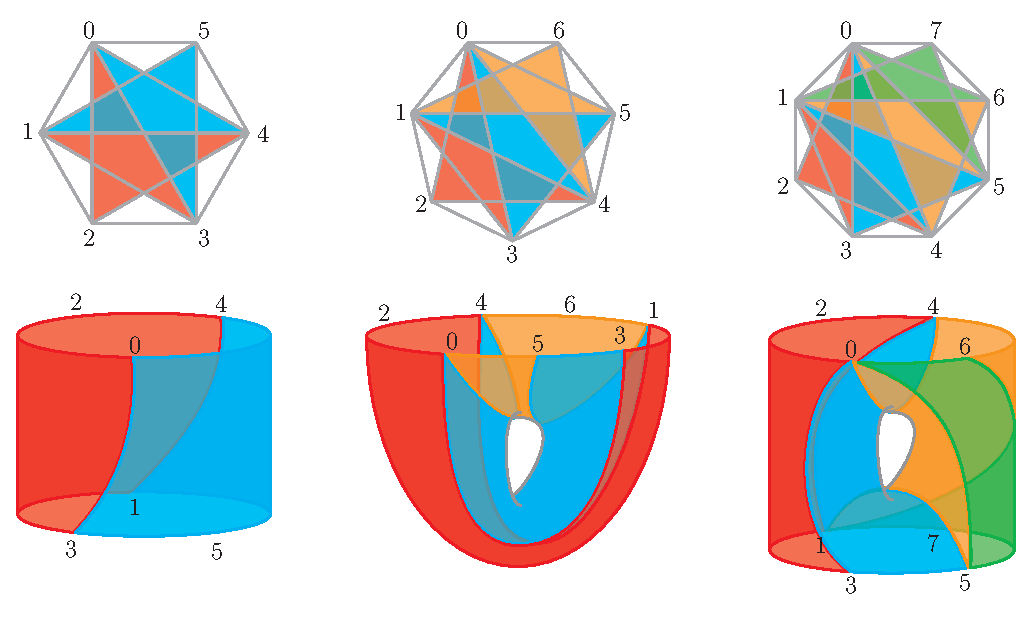
\includegraphics[scale=.7]{surfaces.eps}}
\caption{\small{Examples of decompositions of surfaces associated to the $2$-trangulations $T_{6,2}^{\min}$, $T_{7,2}^{\min}$ and $T_{8,2}^{\min}$.}}\label{surfaces}
\end{figure}
\end{example}

Let $T$ be a $k$-triangulation of the $n$-gon, and let $f$ be a $k$-relevant edge of $T$. Let $R$ and $S$ be the two $k$-stars of $T$ containing $f$, and let $e$ be the common bisector of $R$ and $S$. Let $X$ and $Y$ be the two $k$-stars of $T\triangle\{e,f\}$ containing $e$.

Then $T\setminus\{f\}$ can be viewed as a decomposition of $\mathcal{S}_{n,k}$ into $n-2k-2$ $(2k+1)$-gons and one $(4k)$-gon, obtained from $\mathcal{C}(T)$ by gluing the two $(2k+1)$-gons corresponding to $R$ and $S$ along the edge $f$. And then $T\triangle\{e,f\}$ is obtained from $T\setminus\{f\}$ by splitting the $(4k)$-gon into the two $(2k+1)$-gons corresponding to $X$ and $Y$.

\begin{example}
In figure \ref{monodromy}, we have drawn the decomposition of the cylinder corresponding to the $2$-triangulation $T_{6,2}^{\min}$. The second $2$-triangulation is obtained from $T_{6,2}^{\min}$ by flipping the edge $[1,4]$, and we have represented the decomposition of the cylinder obtained by flipping the edge on the surface. When flipping similarily $[0,3]$ and then $[2,5]$, we obtain again the triangulation $T_1$. Observe that although the corresponding decomposition is combinatorially the same as in the first picture, it has been twisted on the surface. 

\begin{figure}
\centerline{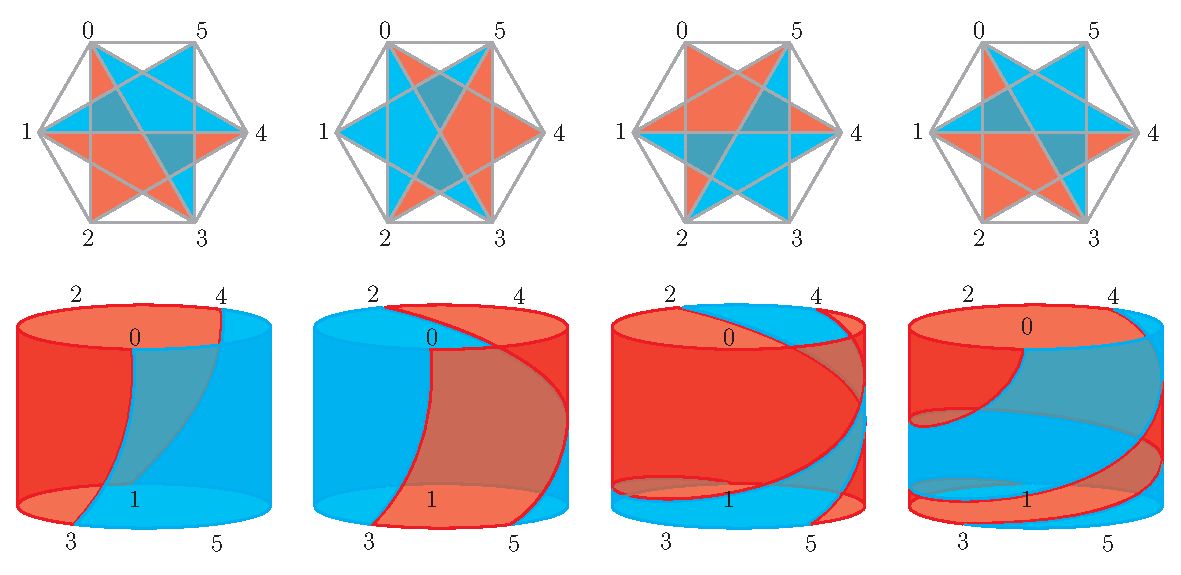
\includegraphics[scale=.7]{monodromy.eps}}
\caption{\small{A cycle of flips.}}\label{monodromy}
\end{figure}
\end{example}

More generaly, there is a morphism between
\begin{enumerate}[(i)]
\item the \emph{fundamental group} $\pi_{n,k}$ of the graph of flips $G_{n,k}$ ({\it i.e.} the set of loops in $G_{n,k}$, up to homotopy), and
\item the \emph{mapping class group} $\mathcal{M}_{n,k}$ of the surface $\mathcal{S}_{n,k}$ ({\it i.e.} the set of diffeomorphisms of the surface $\mathcal{S}_{n,k}$ into itself that preserve the orientation and that fixe the boundary of $\mathcal{S}_{n,k}$, up to isotopy).
\end{enumerate}




%%%%%%%%%%%%%%%%%%%%%%%%%%%%%%%%%%%%%%%%%%%%%%%%%%%%%%%%%


\section{Strongly regular decompositions}\label{sectionregulardecomp}

This section is devoted to an application of multi-triangulations to the construction of strongly regular polygonal decompositions of surfaces of high genus. The main result is the following:

\begin{proposition}\label{decomp}
For any positive integers $\ell$ and $m$, there exists a polygonal decomposition of the closed surface of genus 
$$g=(\ell-1)(\ell^2m^2-\frac{\ell m}{2}-1)$$
into $(2\ell m+1)$-gons with $\ell(2\ell m+1)$ vertices, $\ell(\ell m-m+1)(2\ell m+1)$ edges and $2\ell(\ell m-m+1)$ polygons, such that
\begin{enumerate}
\item all the vertices have the same degree $2(\ell m-m+1)$,
\item the decomposition is \emph{strongly regular} ({\it i.e.} the vertices (resp. edges) of any polygon are all distincts and two polygons do not share more than one edge).
\end{enumerate}
\end{proposition}


Let $\ell$ and $m$ be two positive integers. Let $k=\ell m$  and $n=\ell(2\ell m+1)$.
Let $Z$ be the set of $k$-relevant edges of $E_n$ defined by
\begin{eqnarray*}
Z & = & \left\{[q-1,-q-k]\;|\; 1\le q\le \lfloor n/2-k\rfloor\right\}\\
&&\cup\left\{[q,-q-k]\;|\; 1\le q\le \lfloor (n-1)/2-k\rfloor\right\}.
\end{eqnarray*}
We call \emph{$k$-zigzag} of $E_n$ any rotation or reflection of $Z$ (see fig. \ref{zigzags}). As we saw in the proof of lemma \ref{diamin}, the union of $k$ disjoint $k$-zigzags of $E_n$ is the set of $k$-relevant edges of a $k$-triangulation. Here, we construct a special as follows.

Let $\rho$ be the rotation $t\mapsto t+2k+1$,  let $\theta$ be the rotation $t\mapsto t+2$ and let $\sigma$ be the reflection $t\mapsto -t$. Let $\Gamma$ denote the dihedral group of order $2\ell$ generated by $\rho$ and $\sigma$.

\begin{lemma}
The set
$$\bigcup_{i=0}^{m-1} \theta^i\left(\bigcup_{\gamma\in\Gamma} \gamma(Z)\right)$$
is the subset of the $k$-relevant edges of a $k$-triangulation $T$ of the $n$-gon.
\end{lemma}

\begin{proof}
Observe that $Z$ has a stabilizer of cardinality $2$ in $\Gamma$, so that $\bigcup_{\gamma\in\Gamma} \gamma(Z)$ consists of $\ell$ (and not $2\ell$) $k$-zigzags of $E_n$. Indeed,
\begin{enumerate}[(i)]
\item if $\ell$ is odd, then $\sigma(Z)=Z$, and $\bigcup_{\gamma\in\Gamma} \gamma(Z)$ is the disjoint union of the $\ell$ $k$-zigzags $\rho^i(Z)$, for $0\le i\le \ell-1$;
\item if $\ell$ is even, then $\rho^{\ell/2}(Z)=Z$, and $\bigcup_{\gamma\in\Gamma} \gamma(Z)$ is the disjoint union of the $\ell/2$ zigzags $\rho^i(Z)$, for $0\le i\le \ell/2-1$, and the $\ell/2$ zigzags $\rho^i\circ\sigma(Z)$, for $0\le i\le \ell/2-1$.
\end{enumerate}
Consequently, the set $\bigcup_{i=0}^{m-1} \theta^i\left(\bigcup_{\gamma\in\Gamma} \gamma(Z)\right)$ is the disjoint union of $\ell m=k$ $k$-zigzags, with proves the lemma.
\end{proof}

\begin{lemma}\label{A}
The degree of any vertex in $T$ is $2m(2\ell-1)$.
\end{lemma}

\begin{proof}
Any vertex $v$ of $V_n$ is contained in $2(\ell-1)$ edges of $\bigcup_{\gamma\in\Gamma} \gamma(Z)$. Consequently, $v$ is contained in $2m(l-1)$ $k$-relevant edges of $T$. Since it is contained in $2k$ $k$-irrelevant or $k$-boundary edges, the degree of $v$ is $2m(l-1)+2ml=2m(2l-1)$.
\end{proof}

In this stage, we have constructed an infinite familly of multi-triangulations indexed by $\ell$ and $m$. The corresponding polygonal complex $\mathcal{C}(T)$ is a decomposition of $\mathcal{S}_{n,k}$ into $(2k+1)$-gons with constant vertex-degree equal to $2(\ell m-m+1)$ and such that the vertices (resp. edges) of any polygon are all distincts. The two following lemmas prove that in the complex $\mathcal{C}(T)$,
\begin{enumerate}[(i)]
\item a polygon do not have more than one edge in each boundary component of $\mathcal{S}_{n,k}$;
\item two polygons do not share more than one edge.
\end{enumerate}

\begin{lemma}\label{B}
Any $k$-star of $T$ contains at least one and at most two $k$-boundary edges.
\end{lemma}

\begin{proof}
Note first that $T$ does not contain any pair of consecutive edges of length $k+1$. According to lemma \ref{consectivboundary}, this implies that any $k$-star of $T$ contains at most two $k$-boundary edge. Moreover, $T$ contains $2k$ edges of length $k+1$ so that there are exactly $2k$ $k$-stars of $T$ containing two $k$-boundary edges. But then the number of $k$-stars of $T$ containing one $k$-boundary edge is $n-4k$, {\it i.e.} the number of remaining $k$-stars.
\end{proof}

Observe first that this lemma proves (i). Indeed, if a $k$-star contains two $k$-boundary edges, then they are consecutive (lemma \ref{consectivboundary}), and therefore they are not in the same boundary component of $\mathcal{S}_{n,k}$.

Moreover, it ensures that for any $k$-star $S$ of $T$, the set $X(S)=\{v\in V_n\;|\; [v,v+k]\in S\}$ is a non-empty cyclic interval. Consequently, the cyclic order on $V_n$ provides a cyclic order on the $k$-stars of $T$. Label the $k$-stars of $T$ with $\mathbb{Z}_{n-2k}$ according to this order. 


\begin{lemma}\label{C}
Any pair of $k$-stars of $T$ shares at most one edge. 
\end{lemma}

\begin{proof}
IN PROGRESS
\end{proof}

We are now in position to prove proposition \ref{decomp}. 
For any $0\le i\le l-1$, let $P_i$ denote the $(2k+1)$-gon with edges $\{[i+\ell j,i+\ell j+k]\;|\; 0\le j\le 2k\}$ and let $\hat{\mathcal{C}}$ be the polyhedral complex $\mathcal{C}(T)\cup\{P_0,\ldots,P_{\ell-1}\}$. It provides a decomposition of the closed surface of genus 
$$g=(\ell-1)(\ell^2m^2-\frac{\ell m}{2}-1)$$
into $(2k+1)$-gons, with constant vertex-degree equal to $2(\ell m-m+1)$ (lemma \ref{A}) and which is strongly regular (lemmas \ref{B} and \ref{C}).

Observe the following properties of this decomposition:
\begin{enumerate}
\item when $\ell$ (or $m$) is big, the number of edges is equivalent to twice the genus, which is optimal;
\item when $m=1$, the degree of the vertices and the number of edges of the polygons differ just by $1$;
\item when $\ell=2$, we have a strongly regular decomposition of a surface of genus $g$ using $4\sqrt{g}$ vertices of degree $\sqrt{g}$, $2g$ edges, and $2\sqrt{g}$ polygons with $2\sqrt{g}$ edges.
\end{enumerate}

Note furthermore that the triangulation $T$, and thus the corresponding surface decomposition, is invariant by the dihedral group $\Lambda$ of order $2\ell$ generated by $\rho$ and $\tau=\theta^{m-1}\circ\sigma$.


%%%%%%%%%%%%%%%%%%%%%%%%%%%%%%%%%%%%%%%%%%%%%%%%%%%%%%%%%


\section{Further topics and open questions}\label{sectionopen}



In this section, we discuss further topics and open questions related to multi-triangulations that may be easier with the tool of $k$-stars.


\paragraph{{\sc Rigidity}}



\paragraph{{\sc Multi-Dyck paths}}


\paragraph{{\sc Chirotopes}}



\paragraph{{\sc Multi-associahedron}}

%%%%%%%%%%%%%%%%%%%%%%%%%%%%%%%%%%%%%%%%%%%%%%%%%%%%%%%%%


\nocite{j-gtdfssp-05}
\nocite{cp-tttccp-92}
\nocite{i-mcg-02}

\bibliographystyle{alpha}
\bibliography{biblio.bib}




\end{document}
